\documentclass[11pt, oneside]{article}   	% use "amsart" instead of "article" for AMSLaTeX format
\usepackage{geometry}                		% See geometry.pdf to learn the layout options. There are lots.
\geometry{letterpaper}                   		% ... or a4paper or a5paper or ... 
%\geometry{landscape}                		% Activate for rotated page geometry
\usepackage[parfill]{parskip}    		% Activate to begin paragraphs with an empty line rather than an indent

\usepackage[utf8]{inputenc} % Any characters can be typed directly from the keyboard, eg éçñ
\usepackage{textcomp} % provide lots of new symbols
\usepackage{graphicx}  % Add graphics capabilities
%\usepackage{epstopdf} % to include .eps graphics files with pdfLaTeX
\usepackage{flafter}  % Don't place floats before their definition
%\usepackage{topcapt}   % Define \topcation for placing captions above tables (not in gwTeX)
%\usepackage{natbib} % use author/date bibliographic citations %May conflict with some bibliography style download somewhere


\usepackage{amsmath,amssymb}  % Better maths support & more symbols
\usepackage{bm}  % Define \bm{} to use bold math fonts

\usepackage[pdftex,bookmarks,colorlinks,breaklinks]{hyperref}  % PDF hyperlinks, with coloured links
%\definecolor{dullmagenta}{rgb}{0.4,0,0.4}   % #660066
%\definecolor{darkblue}{rgb}{0,0,0.4}
\hypersetup{linkcolor=blue,citecolor=blue,filecolor=dullmagenta,urlcolor=darkblue} % coloured links
%\hypersetup{linkcolor=black,citecolor=black,filecolor=black,urlcolor=black} % black links, for printed output

\usepackage{memhfixc}  % remove conflict between the memoir class & hyperref
% \usepackage[activate]{pdfcprot}  % Turn on margin kerning (not in gwTeX)
% \usepackage{pdfsync}  % enable tex source and pdf output syncronicity

\usepackage{array}%for table width
\newcolumntype{L}[1]{>{\raggedright\let\newline\\\arraybackslash\hspace{0pt}}m{#1}}
\newcolumntype{C}[1]{>{\centering\let\newline\\\arraybackslash\hspace{0pt}}m{#1}}
\newcolumntype{R}[1]{>{\raggedleft\let\newline\\\arraybackslash\hspace{0pt}}m{#1}}

\usepackage{caption}%Add captions to figures

\usepackage{booktabs}%For \toprule \midrule \bottomrule

\usepackage{multicol}%Create multicolumns in report
\usepackage{wrapfig}%Insert floating elements into multicolumns in report
\usepackage{float}%To use placement specifier H in float element of figure
\usepackage{longtable}%required by longtabu
\usepackage{tabu}%Build a table span several pages
\usepackage{tabularx}%Control and adjust the width of columns in tabulars
\usepackage{listings}%Include code into latex
\usepackage{color}

\usepackage{pgfplotstable}% Include excel file into latex

\usepackage{tikz}%Package for drawing graphical models
\usetikzlibrary{shapes, arrows, calc, positioning,matrix}
\tikzset{
data/.style={circle, draw, text centered, minimum height=3em ,minimum width = .5em, inner sep = 2pt},
empty/.style={circle, text centered, minimum height=3em ,minimum width = .5em, inner sep = 2pt},
}
 
\definecolor{codegreen}{rgb}{0,0.6,0}
\definecolor{codegray}{rgb}{0.5,0.5,0.5}
\definecolor{codepurple}{rgb}{0.58,0,0.82}
\definecolor{backcolour}{rgb}{0.95,0.95,0.92}

\lstdefinestyle{mystyle}{
    backgroundcolor=\color{backcolour},   
    commentstyle=\color{codegreen},
    keywordstyle=\color{magenta},
    numberstyle=\tiny\color{codegray},
    stringstyle=\color{codepurple},
    basicstyle=\footnotesize,
    breakatwhitespace=false,         
    breaklines=true,                 
    captionpos=b,                    
    keepspaces=true,                 
    numbers=left,                    
    numbersep=5pt,                  
    showspaces=false,                
    showstringspaces=false,
    showtabs=false,                  
    tabsize=2
}
 
\lstset{style=mystyle}

\DeclareCaptionFont{white}{\color{white}}
\DeclareCaptionFormat{listing}
     {\parbox{\dimexpr\textwidth-4\fboxsep}{\centering #1#2#3}}
\captionsetup[lstlisting]{format=listing}
%\captionsetup[lstlisting]{format=listing,labelfont=white,textfont=white}

\usepackage{enumerate}

\usepackage{fancyvrb}%include a txt file into latex pdf

\usepackage{seqsplit}
\newcommand\foo[2]{%
    \begin{minipage}{#1}
    \seqsplit{#2}
    \end{minipage}
    }

%newcommand
\newcommand{\notimplies}{%
  \mathrel{{\ooalign{\hidewidth$\not\phantom{=}$\hidewidth\cr$\implies$}}}}

%\usepackage[utf8]{inputenc}
%\usepackage[english]{babel}
%\usepackage{amsmath}
%\usepackage{amsfonts}
%\usepackage{amssymb}
%\usepackage{amsbsy}
%\usepackage{bm}
%\usepackage{fixmath}
%\usepackage{makeidx}
%\usepackage{graphicx}
%
%\usepackage{array}%for table width
%\newcolumntype{L}[1]{>{\raggedright\let\newline\\\arraybackslash\hspace{0pt}}m{#1}}
%\newcolumntype{C}[1]{>{\centering\let\newline\\\arraybackslash\hspace{0pt}}m{#1}}
%\newcolumntype{R}[1]{>{\raggedleft\let\newline\\\arraybackslash\hspace{0pt}}m{#1}}
%
%\usepackage{grffile}%avoid showing file name when including a file
%\usepackage{verbatim}%include code as appendix
%\usepackage[left=1in,right=1in,top=1in,bottom=0.8in]{geometry}
%
%\usepackage{array}
%
%\usepackage{pdfpages}%for including pdf of R-code
%
%\setlength\parindent{0pt}%noindent
%
%
%
%\DeclareMathOperator{\Tr}{Tr}

\DeclareMathOperator*{\argmin}{argmin}


\title{HW1-ECON-482}
\author{Kungang Zhang}
\date{October 27, 2016}							% Activate to display a given date or no date

\begin{document}
\maketitle
\section{Prob 1:}
\begin{enumerate}[(1)]
\item
According to the statement, we use flat prior, so that maximizing the posterior is equivalent to maximizing likelihood (``conditional likelihood" given the initial data). There are two ways to do prediction:
\begin{itemize}
\item
Moving window:
\begin{table}[!ht]
\center
\captionsetup{width=0.8\textwidth}
\begin{tabularx}{0.8\textwidth}{c c c c c c} 
 $[~1,$ & $2,\cdots,$ & $T,\cdots,$ & $T+h~]$ & &\\  
 & $[2,\cdots,$ & $T,\cdots,$ & $T+h,$ & $T+h+1~]$ &\\
 & & $\cdots$ & $\cdots$& $\cdots$& \\
 & & $[T,\cdots,$ & $T+h,$ & $T+h+1,\cdots,$ & $2T+h-1~]$ \\ 
 & & & $\cdots$ & $\cdots$& $\cdots$\\
 \end{tabularx} 
\end{table}
\item
Extending window:
\begin{table}[!ht]
\center
\captionsetup{width=0.8\textwidth}
\begin{tabularx}{0.8\textwidth}{c c c c c c} 
 $[~1,$ & $2,\cdots,$ & $T,\cdots,$ & $T+h~]$ & &\\  
 $[~1,$ & $2,\cdots,$ & $T,\cdots,$ & $T+h,$ & $T+h+1~]$ &\\
 & & $\cdots$ & $\cdots$& $\cdots$& \\
 $[~1,$ & $2,\cdots,$ & $T,\cdots,$ & $T+h,$ & $T+h+1,\cdots,$ & $2T+h-1~]$ \\ 
 & & & $\cdots$ & $\cdots$& $\cdots$\\
 \end{tabularx} 
\end{table}
\end{itemize}

Here I tried both cases and get the MSFE:
\begin{table}[!ht]
\center
\captionsetup{width=0.8\textwidth}
\begin{tabularx}{0.8\textwidth}{|X|X|X|X|X|} \hline 
MSFE & log-real GDP & log-real GDP & log-GDP deflator & log-GDP deflator \\ \hline
 Average growth rate & 1 quarter & 4 quarters & 1 quarter & 4 quarters \\ \hline
 Moving window & $2.500e-3$ & $3.872e-4$ & $1.374e-3$ & $4.272e-4$	\\ \hline
 Extending window & $1.919e-3$ & $2.195e-4$ & $1.246e-3$ & $2.289e-4$ \\ \hline 
 \end{tabularx} 
\caption{Mean squared forecast error for moving window and extending window.}
\label{table:MSFE_flat_pri}
\end{table}

According to Table \ref{table:MSFE_flat_pri}, looks like the extending window method has smaller MSFE.

\item
According to \cite{giannone2016priors}, with Minnesota prior as specified, the posterior would looks like:
\begin{align}
\beta | \Sigma, Y & \sim \mathcal{N} (\hat{ \beta}, \Sigma \otimes \Omega) \\
\hat {B} &= (X^TX+ \Omega ^{-1}) ^{-1} (X^TY + \Omega ^{-1} \hat{b}) \\
\hat { \beta} & = vec[ \hat {B}] \\
b & = vec[\hat {b}]
\end{align}
\begin{align}
 \Omega = &\lambda^2 
 \begin{bmatrix}
 10^6 & &  & & &  0 &&\\
 & \frac{1}{\hat{ \sigma}^2_1}& &  0& & & &  &\\
  & & \ddots & & & & & \\
  & & & \frac{1}{\hat{ \sigma}_M^2} & && & &0&\\
  & & & &\frac{2 ^{-2}}{\hat{ \sigma}_1^2} &  &0& &\\
    & & & & &\ddots  && &\\
    & & & & &  &\frac{2 ^{-2}}{\hat{ \sigma}_M^2}& & &\\
    & & & & &  & &\ddots & & \\
\end{bmatrix} _{K\times K} \\
b =& ([0,1,0,\cdots,0| 0,0,1,0,\cdots,0|\cdots]^T )_{K \times 1}\\
\hat { \sigma}_i^2 = & \frac{1}{T}\sum_{t=1}^{T} \left[ (y _{i,t}- \hat {c}_i - \hat { \phi}_iy _{i,t-1}) ^{2} \right] \nonumber \\
=& \frac{1}{T}\sum_{t=1}^{T} (y _{i,t}^2+\hat {c}_i^2 + \hat { \phi}_i^2 y _{i,t-1}^2+2\hat {c}_i \hat { \phi}_i y _{i,t-1}- 2\hat {c}_i y _{i,t}-2\hat { \phi}_i y _{i,t-1} y _{i,t})\\ 
 \begin{bmatrix}
 \hat {c}_i \\
 \hat { \phi}_i \\
\end{bmatrix} =&
\begin{bmatrix}
 T & \sum_{t = 1}^{T} y _{i,t-1} \\
 \sum_{t = 1}^{T} y _{i,t-1} & \sum_{t = 1}^{T} y _{i,t-1}^2 \\
\end{bmatrix} ^{-1}
\begin{bmatrix}
\sum_{t = 1}^{T} y _{i,t} \\
\sum_{t=1}^{T} y _{i,t-1} y _{i,t}\\
\end{bmatrix}
\end{align}
where $K = Mp + 1$, $M = dim(y)$, $p = max~time~lag$, and the given observations are $y _{-p+1},\cdots,y _{0}$ and the values to forecast are $y_1,\cdots,y_T$. Part of these expressions come from \cite{hamilton1994time}, Section 5.2. The last two equation mean the parameters $\hat { \sigma}_i^2$ are MLE based on $AR(1)$ model, given $y _{i,0}$.
Here, we don't need to know $ \Sigma$ because we only need a point estimation of $\hat { \beta}$. Using the same procedure as in (1), we get the MSFE as:
\begin{table}[!ht]
\center
\captionsetup{width=0.8\textwidth}
\begin{tabularx}{0.8\textwidth}{|X|X|X|X|X|} \hline 
MSFE & log-real GDP & log-real GDP & log-GDP deflator & log-GDP deflator \\ \hline
 Average growth rate & 1 quarter & 4 quarters & 1 quarter & 4 quarters \\ \hline
 Extending window & $9.387e-4$ & $1.493e-4$ & $5.444e-4$ & $1.856e-4$ \\ \hline 
 \end{tabularx} 
\caption{Mean squared forecast error for moving window and extending window.}
\label{table:MSFE_minne_prior}
\end{table}
The MSFE for Minnesota priors for 1 quarter forecast is smaller than that for flat prior, but the MSEF for Minnesota priors for 4 quarter forecast is larger.

\item
The marginal likelihood is (as shown in \cite{giannone2016priors} and its supplemental file):
\begin{align}
P (y| \lambda) = &(\frac{1}{ \pi}) ^{\frac{MT}{2}} \frac{ \Gamma _{M} (\frac{T+d}{2})}{ \Gamma _{M} (\frac{d}{2})}| \Omega| ^{-\frac{M}{2}} | \Psi| ^{\frac{d}{2}} |X^TX + \Omega ^{-1}| ^{-\frac{M}{2}} \nonumber \\   &* | \Psi + \hat { \epsilon}^T\hat { \epsilon} + (\hat {B}-\hat {b})^T \Omega ^{-1}(\hat {B}-\hat {b})| ^ {-\frac{T+d}{2}} \label{eqn:MMLE}\\
\hat { \epsilon} =& Y - X\hat {B} \nonumber
\end{align}
Maximizing the posterior with flat prior is equivalent to maximizing the marginal likelihood. By using notation $E _{ \Psi}E _{ \Psi}^T = \Psi ^{-1}$, $D _{ \Omega}D _{ \Omega}^T = \Omega$, and $ \lambda^2 \Phi = \Omega$ or $ \lambda D _{ \Phi} = D _{ \Omega}$ , the \ref{eqn:MMLE} can be simplified as:
\begin{align}
P (y| \lambda) = &(\frac{1}{ \pi}) ^{\frac{MT}{2}} \frac{ \Gamma _{M} (\frac{T+d}{2})}{ \Gamma _{M} (\frac{d}{2})} | \Psi| ^{-\frac{T}{2}} \left|D _{ \Omega}^TX^TXD _{ \Omega} + I _{K}\right| ^{-\frac{M}{2}} \nonumber \\   &* \left| I_{M} + E _{ \Psi}^T\left[ \hat { \epsilon}^T\hat { \epsilon} + (\hat {B}-\hat {b})^T \Omega ^{-1}(\hat {B}-\hat {b})\right ] E _{ \Psi} \right| ^ {-\frac{T+d}{2}} \nonumber \\
\propto & \left| \lambda^2 D _{ \Phi}^TX^TXD _{ \Phi} + I _{K}\right| ^{-\frac{M}{2}} \nonumber \\   &* \left| \lambda^2 I_{M} + E _{ \Psi}^T\left[ \lambda^2 \hat { \epsilon}^T\hat { \epsilon} + (\hat {B}-\hat {b})^T \Phi ^{-1}(\hat {B}-\hat {b})\right ] E _{ \Psi} \right| ^ {-\frac{T+d}{2}} \lambda ^{M(T+d)} \label{eqn:MMLE_sim} \\
\hat { \epsilon}^T\hat { \epsilon} =& (Y-X\hat {B})^T(Y-X\hat {B}) \nonumber \\
\hat {B} = & (\lambda^2X^TX+ \Phi ^{-1}) ^{-1} (\lambda^2 X^TY + \Phi ^{-1} \hat{b}) \nonumber
\end{align}
We can use gradient method to optimize \ref{eqn:MMLE_sim}. First we take log and then take derivative w.r.t. $\lambda$. However, the code to implement this would be much more complex. Here, I just use grid-search first. 
The MSFE depends on the interval we specify to do grid search.
\begin{table}[!ht]
\center
\captionsetup{width=0.8\textwidth}
\begin{tabularx}{0.8\textwidth}{|X|X|X|X|X|} \hline 
MSFE & log-real GDP & log-real GDP & log-GDP deflator & log-GDP deflator \\ \hline
 Average growth rate & 1 quarter & 4 quarters & 1 quarter & 4 quarters \\ \hline
 $[0.0001,1]$ & $9.524e-4$ & $1.748e-4$ & $5.020e-4$ & $2.014e-4$ \\ \hline 
  $[0.05,1]$ & $9.063e-4$ & $1.604e-4$ & $4.995e-4$ & $1.934e-4$ \\ \hline 
 \end{tabularx} 
\caption{Mean squared forecast error for moving window and extending window.}
\label{table:MSFE_minne_prior}
\end{table}
\begin{figure}[!ht]
\begin{center}
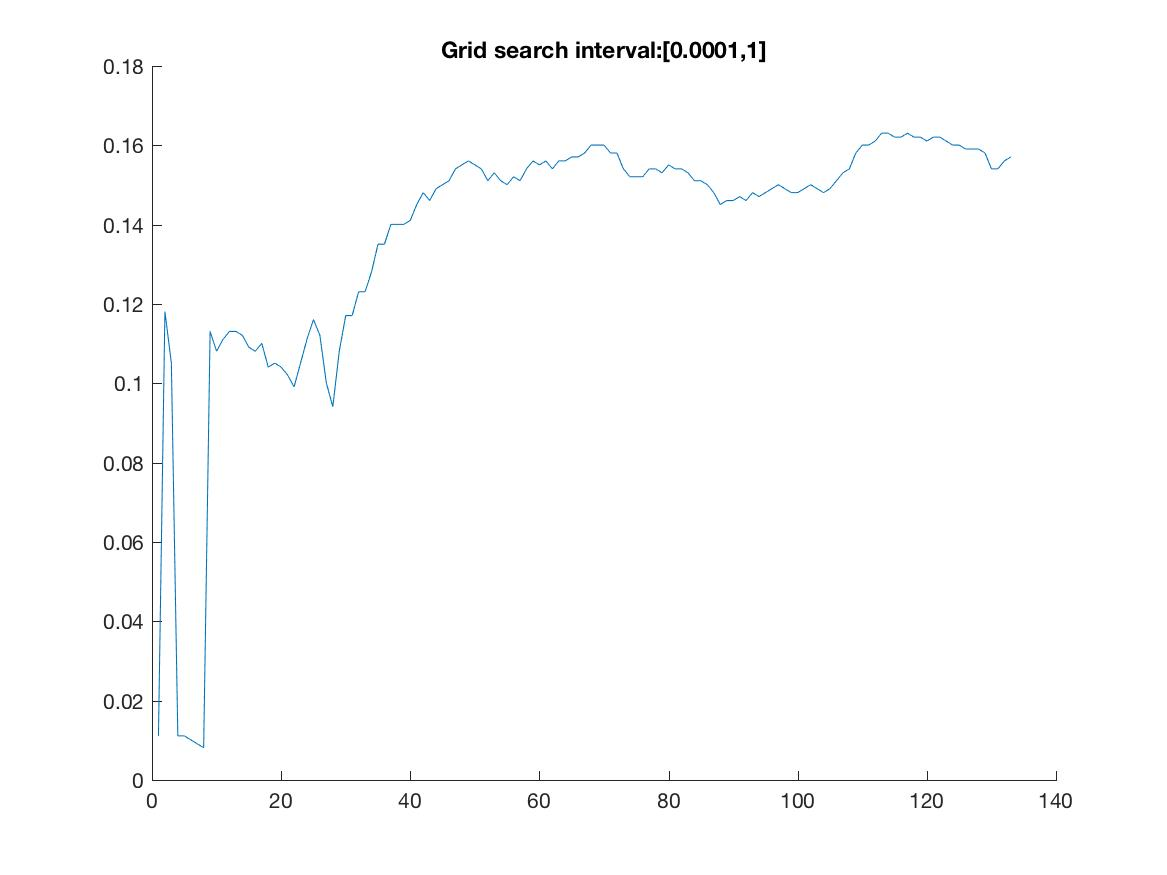
\includegraphics[width = 0.45\textwidth]{lambda_opt_1.jpg}
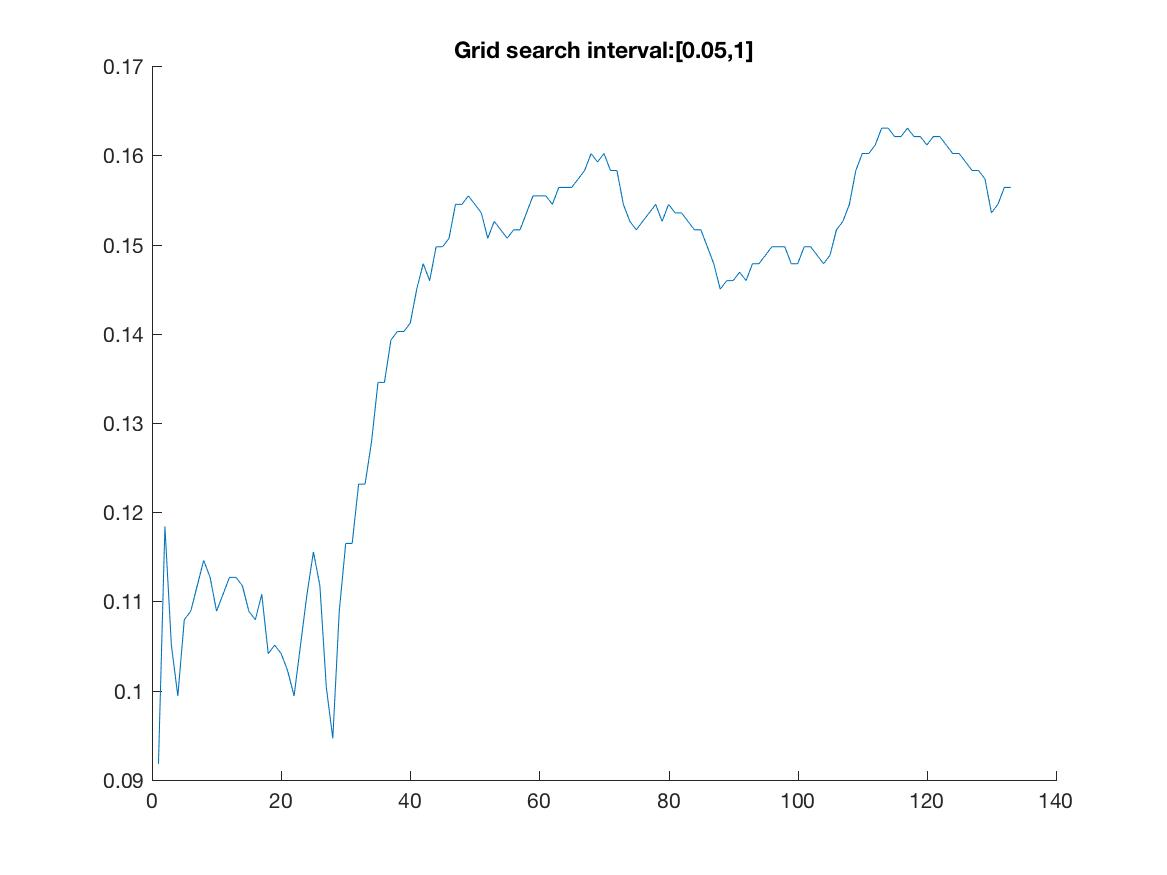
\includegraphics[width = 0.45\textwidth]{lambda_opt_2.jpg}
\captionsetup{width=0.8\textwidth}
\caption{The optimal $ \lambda$ with extending windows and two different search intervals. I am not sure why when $ \lambda$ is near $0$ the path has a big jump. From MSFE, we see they are comparable with those obtained by setting $ \lambda = 0.2$.}
\label{fig:opt_lambda}
\end{center}
\end{figure}
\end{enumerate}


\section{Prob 2:}
\begin{enumerate}[(1)]
\item
First use the whole data set to get MLE for parameters by maximizing likelihood (conditional likelihood conditioning on the first $p$ observations). Then, use the obtained coefficients to do projection from $p+1$ to $T$, based on the given initial observations and later projected values.

\pgfplotstabletypeset[
    col sep=comma,
    string type,
    columns/Name/.style={column name=Name, column type={|l}},
    columns/Observed data/.style={column name=Observed data, column type={|c}},
    columns/Flat prior/.style={column name=Flat prior, column type={|c}},
    columns/Minnesota prior/.style={column name=Minnesota prior, column type={|c}},
    columns/SOC (1)/.style={column name=SOC (1), column type={|c}},
    columns/SOC (5)/.style={column name=SOC (5), column type={|c|}},
    every head row/.style={before row=\hline,after row=\hline},
    every last row/.style={after row=\hline},
    ]{variance.csv}
   
As shown in above form, the variance for log-real GDP, log-labor share, and log-consumption ratio are mostly explained by the deterministic components, but for quarterly price inflation, federal funds rate, and quarterly wage inflation, most of variance cannot be explained by the deterministic components. I think it makes sense because the former three variables are more stable, while the later three variables can be easily affected by the time and current economical situation.
\item
Repeat the same exercise for Minnesota priors.

The difference is very small. They are comparable.
\item
Repeat the same exercise for SOC priors.

The plot is following:
\begin{figure}[!ht]
\begin{center}
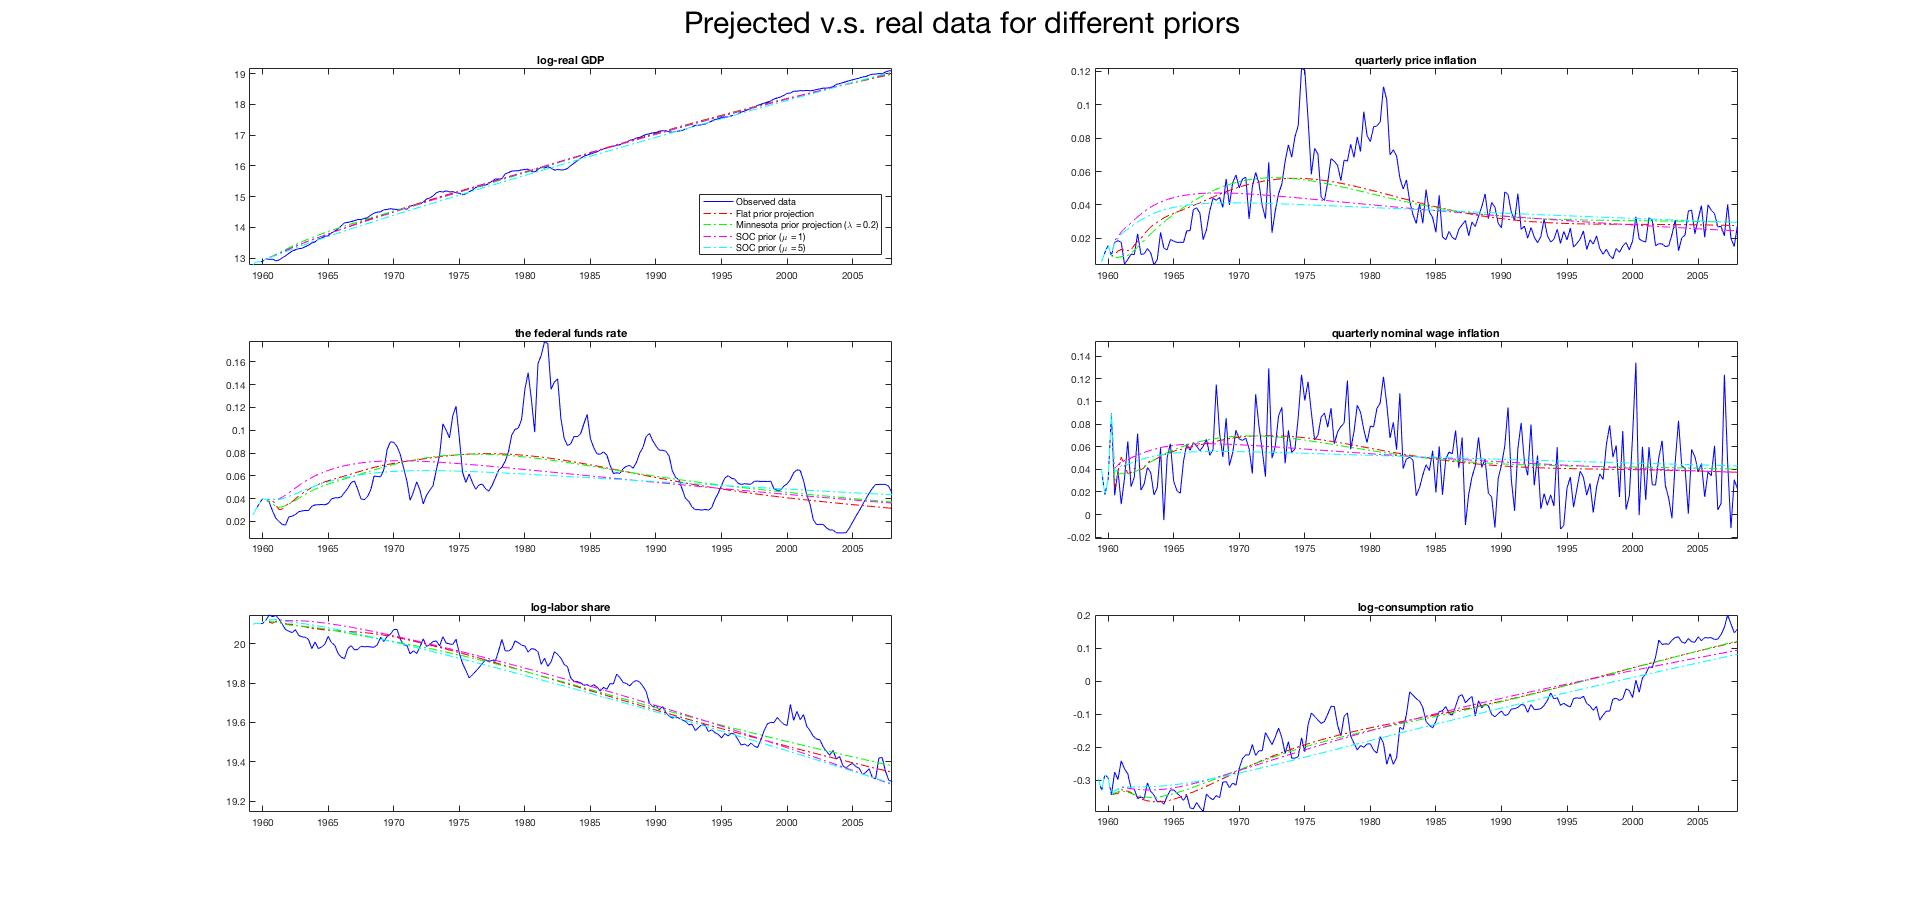
\includegraphics[width = 1.0\textwidth]{part2.jpg}
\captionsetup{width=0.8\textwidth}
\caption{The projections based on the whole data set with flat prior, Minnesota prior, SOC with $ \mu=1$, and SOC with $ \mu=5$.}
\end{center}
\end{figure}
\end{enumerate}
Different priors give very similar results.


\begin{lstlisting}[language=Matlab ,caption={Matlab code for problem 1.}, label={code:prob1}]
clear();
% Load data into the working space
load('dataVARmedium','-mat');
p = 5;
T = 64-5;
N = size(y,1);
M = 7;
K = M*p+1;
h = 4;

%% (1) OLS solution for prediction
%% Moving window prediction
tic
z_comp = zeros(N-(T+p+h)+1,8); % the first four columns are predicted z (average growth rate of GDP) and the second four columns is the real z
for i = 1:(N-(T+p+h)+1)
    % design matrix
    X = zeros(T,K);% a T*K matrix
    for j = 1:T
        X(j,:) = [1,reshape(y((i+j+p-2:-1:i+j-1),:)',1,K-1)];% have to transpose because the reshape function operate in column
    end
    % OLS solution for coefficients
    B_hat = (X'*X)\X'*y((i+p:i+p+T-1),:);% a K*M matrix
    % for h = 1 & 4
    pred_y = zeros(h,M);% a h*M matrix
    y_lag = [1,reshape(y(i+p+T-1:-1:i+T,:)',1,K-1)];% lag of y for the prediction
    for k = 1:h
        % forecast
        pred_y(k,:) = y_lag*B_hat;
        if k<h
            % reform the lag for y of prediction
            y_lag = [1,reshape(pred_y(k:-1:1,:)',1,k*M),reshape(y(i+p+T-1:-1:i+T+k,:)',1,K-1-k*M)];
        end
    end
    z_comp(i,1:2) = pred_y(1,1:2)-y(i+p+T-1,1:2);%predicted average growth rates for one quarter of (i) log-real GDP and (ii) log-GDP delector
    z_comp(i,3:4) = (pred_y(h,1:2)-y(i+p+T-1,1:2))/h;%predicted average growth rates for h quarters of (i) log-real GDP and (ii) log-GDP delector
    z_comp(i,5:6) = y(i+p+T,1:2)-y(i+p+T-1,1:2);%average growth rates for one quarter of (i) log-real GDP and (ii) log-GDP delector
    z_comp(i,7:8) = (y(i+p+T+h-1,1:2)-y(i+p+T-1,1:2))/h;%average growth rates for h quarters of (i) log-real GDP and (ii) log-GDP delector
end
% Calculate the average squared forecast error
MSFE1 = sum((z_comp(:,1:4)-z_comp(:,5:8)).^2,1)/size(z_comp,1)
csvwrite('mse_ex1-1-moving.csv',MSFE1)
toc
%% Expanding window prediction
tic
z_comp = zeros(N-(T+p+h)+1,8); % the first four columns are predicted z (average growth rate of GDP) and the second four columns is the real z
for i = 1:(N-(T+p+h)+1)
    if i ==1
        % design matrix
        X = zeros(T,K);% a T*K matrix
        for j = 1:T
            X(j,:) = [1,reshape(y((j+p-1:-1:j),:)',1,K-1)];% have to transpose because the reshape function operate in column
        end
    else
        new_row = [1,reshape(y((i+T+p-2:-1:i+T-1),:)',1,K-1)];
        X = [X;new_row]; % a (T+i-1)*K matrix
    end
    % OLS solution for coefficients
    B_hat = (X'*X)\X'*y((p+1:p+T+i-1),:);% a K*M matrix
    % for h = 1 & 4
    pred_y = zeros(h,M);% a h*M matrix
    y_lag = [1,reshape(y(T+i+p-1:-1:T+i,:)',1,K-1)];% lag of y for the prediction
    for k = 1:h
        % forecast
        pred_y(k,:) = y_lag*B_hat;
        if k<h
            % reform the lag for y of prediction
            y_lag = [1,reshape(pred_y(k:-1:1,:)',1,k*M),reshape(y(T+i+p-1:-1:T+i+k,:)',1,K-1-k*M)];
        end
    end
    z_comp(i,1:2) = pred_y(1,1:2)-y(i+p+T-1,1:2);%predicted average growth rates for one quarter of (i) log-real GDP and (ii) log-GDP delector
    z_comp(i,3:4) = (pred_y(h,1:2)-y(i+p+T-1,1:2))/h;%predicted average growth rates for h quarters of (i) log-real GDP and (ii) log-GDP delector
    z_comp(i,5:6) = y(i+p+T,1:2)-y(i+p+T-1,1:2);%average growth rates for one quarter of (i) log-real GDP and (ii) log-GDP delector
    z_comp(i,7:8) = (y(i+p+T+h-1,1:2)-y(i+p+T-1,1:2))/h;%average growth rates for h quarters of (i) log-real GDP and (ii) log-GDP delector
end
% Calculate the average squared forecast error
MSFE2 = sum((z_comp(:,1:4)-z_comp(:,5:8)).^2,1)/size(z_comp,1)
csvwrite('mse_ex1-1-extending.csv',MSFE2)
toc
%% (2)Minnesota prior with a given lambda
%% Expanding window prediction
tic
z_comp = zeros(N-(T+p+h)+1,8); % the first four columns are predicted z (average growth rate of GDP) and the second four columns is the real z
% Given lambda
lam = 0.2;
% Estimate b
b_hat = [zeros(M,1),eye(M,M*p)];
for i = 1:(N-(T+p+h)+1)
    if i ==1
        % design matrix
        X = zeros(T,K);% a T*K matrix
        for j = 1:T
            X(j,:) = [1,reshape(y((j+p-1:-1:j),:)',1,K-1)];% have to transpose because the reshape function operate in column
        end
    else
        new_row = [1,reshape(y((i+T+p-2:-1:i+T-1),:)',1,K-1)];
        X = [X;new_row]; % a (T+i-1)*K matrix
    end
    % Estimate elements of Omega
    % The first observation is given (regarded as index 0) and the rest of observation up to the
    % end of current window (index 1 to T) are for prediction as stated in the problem
    % statement
    % Follow Hamilton 1994 to get the MLE for variance
    sum1 = sum(y(1:p+T+i-2,:),1);%sum_1^T y_(t-1)
    sum2 = sum(y(2:p+T+i-1,:),1);%sum_1^T y_(t)
    sum3 = sum(y(1:p+T+i-2,:).^2,1);%sum_1^T y_(t-1)^2
    sum4 = sum(y(2:p+T+i-1,:).^2,1);%sum_1^T y_(t)^2
    sum5 = sum(y(2:p+T+i-1,:).*y(1:p+T+i-2,:),1);%sum_1^T y_(t)y_(t-1)
    sigma2_hat = zeros(1,M);
    for m = 1:M
        c_phi_hat = [p+T+i-2,sum1(m);sum1(m),sum3(m)]\[sum2(m);sum5(m)];% c_phi_hat = [c_hat,phi_hat]
        sigma2_hat(m) = 1.0/(p+T+i-2)*(sum4(m)+c_phi_hat(2)^2*sum3(m)+2*c_phi_hat(1)*c_phi_hat(2)*sum1(m)...
                        -2*c_phi_hat(1)*sum2(m)-2*c_phi_hat(2)*sum5(m))+c_phi_hat(1)^2;
    end
    omega_d = [10^6];
    for j = 1:p
        omega_d = [omega_d,(sigma2_hat*j^2).^(-1)];
    end
    % Times the lambda^2
    omega_d = lam^2 * omega_d;
    % MAP solution for coefficients
    B_hat = (X'*X+diag(omega_d.^(-1)))\(X'*y((p+1:p+T+i-1),:)+diag(omega_d.^(-1))*b_hat');% a K*M matrix
    % for h = 1 & 4
    pred_y = zeros(h,M);% a h*M matrix
    y_lag = [1,reshape(y(T+i+p-1:-1:T+i,:)',1,K-1)];% lag of y for the prediction
    for k = 1:h
        % forecast
        pred_y(k,:) = y_lag*B_hat;
        if k<h
            % reform the lag for y of prediction
            y_lag = [1,reshape(pred_y(k:-1:1,:)',1,k*M),reshape(y(T+i+p-1:-1:T+i+k,:)',1,K-1-k*M)];
        end
    end
    z_comp(i,1:2) = pred_y(1,1:2)-y(i+p+T-1,1:2);%predicted average growth rates for one quarter of (i) log-real GDP and (ii) log-GDP delector
    z_comp(i,3:4) = (pred_y(h,1:2)-y(i+p+T-1,1:2))/h;%predicted average growth rates for h quarters of (i) log-real GDP and (ii) log-GDP delector
    z_comp(i,5:6) = y(i+p+T,1:2)-y(i+p+T-1,1:2);%average growth rates for one quarter of (i) log-real GDP and (ii) log-GDP delector
    z_comp(i,7:8) = (y(i+p+T+h-1,1:2)-y(i+p+T-1,1:2))/h;%average growth rates for h quarters of (i) log-real GDP and (ii) log-GDP delector
end
% Calculate the average squared forecast error
MSFE3 = sum((z_comp(:,1:4)-z_comp(:,5:8)).^2,1)/size(z_comp,1)
csvwrite('mse_ex1-1-lambda_given.csv',MSFE3)
toc
%% (3)Minnesota prior without a given lambda (optimize marginal likelihood to get lambda each time)
%% Expanding window prediction
tic
%Cannot set lambda = 0, because when take log of lambda, 0 is not
%meaningful
lam_bd = [0.0001,1];
N_try = 1000;
d = M + 2;
z_comp = zeros(N-(T+p+h)+1,8); % the first four columns are predicted z (average growth rate of GDP) and the second four columns is the real z
% Record optimal value of lambda
rec_lam_opt = zeros(N-(T+p+h)+1,1);
% Estimate b
b_hat = [zeros(M,1),eye(M,M*p)];
for i = 1:(N-(T+p+h)+1)
    if i ==1
        % design matrix
        X = zeros(T,K);% a T*K matrix
        for j = 1:T
            X(j,:) = [1,reshape(y((j+p-1:-1:j),:)',1,K-1)];% have to transpose because the reshape function operate in column
        end
    else
        new_row = [1,reshape(y((i+T+p-2:-1:i+T-1),:)',1,K-1)];
        X = [X;new_row]; % a (T+i-1)*K matrix
    end
    % Estimate elements of Omega
    % The first observation is given and the rest of observation up to the
    % end of current window are for prediction as stated in the problem
    % statement
    % Follow Hamilton 1994 to get the MLE for variance
    sum1 = sum(y(1:p+T+i-2,:),1);%sum_1^T y_(t-1)
    sum2 = sum(y(2:p+T+i-1,:),1);%sum_1^T y_(t)
    sum3 = sum(y(1:p+T+i-2,:).^2,1);%sum_1^T y_(t-1)^2
    sum4 = sum(y(2:p+T+i-1,:).^2,1);%sum_1^T y_(t)^2
    sum5 = sum(y(2:p+T+i-1,:).*y(1:p+T+i-2,:),1);%sum_1^T y_(t)y_(t-1)
    sigma2_hat = zeros(1,M);
    for m = 1:M
        c_phi_hat = [p+T+i-2,sum1(m);sum1(m),sum3(m)]\[sum2(m);sum5(m)];% c_phi_hat = [c_hat,phi_hat]
        temp_sum = 0;
        sigma2_hat(m) = 1.0/(p+T+i-2)*(sum4(m)+c_phi_hat(2)^2*sum3(m)+2*c_phi_hat(1)*c_phi_hat(2)*sum1(m)...
                        -2*c_phi_hat(1)*sum2(m)-2*c_phi_hat(2)*sum5(m))+c_phi_hat(1)^2;
    end
    omega_d = [10^6];
    for j = 1:p
        omega_d = [omega_d,(sigma2_hat*j^2).^(-1)];
    end
    % Optimize in terms of lambda
    % Use grid-search method
    %options_optim = optimoptions(@fminunc,'Display','iter-detailed','Algorithm','quasi-newton','SpecifyObjectiveGradient',true,'MaxIterations',1000);
    rec_lam_opt(i) = lam_mle_grid(@logmlikelih,lam_bd,N_try,X,y((p+1:p+T+i-1),:),sigma2_hat,omega_d,b_hat',M,T+i-1,d);
    % Times the lambda^2
    omega_d = rec_lam_opt(i)^2 * omega_d;
    % MAP solution for coefficients
    B_hat = (X'*X+diag(omega_d.^(-1)))\(X'*y((p+1:p+T+i-1),:)+diag(omega_d.^(-1))*b_hat');% a K*M matrix
    % for h = 1 & 4
    pred_y = zeros(h,M);% a h*M matrix
    y_lag = [1,reshape(y(T+i+p-1:-1:T+i,:)',1,K-1)];% lag of y for the prediction
    for k = 1:h
        % forecast
        pred_y(k,:) = y_lag*B_hat;
        if k<h
            % reform the lag for y of prediction
            y_lag = [1,reshape(pred_y(k:-1:1,:)',1,k*M),reshape(y(T+i+p-1:-1:T+i+k,:)',1,K-1-k*M)];
        end
    end
    z_comp(i,1:2) = pred_y(1,1:2)-y(i+p+T-1,1:2);%predicted average growth rates for one quarter of (i) log-real GDP and (ii) log-GDP delector
    z_comp(i,3:4) = (pred_y(h,1:2)-y(i+p+T-1,1:2))/h;%predicted average growth rates for h quarters of (i) log-real GDP and (ii) log-GDP delector
    z_comp(i,5:6) = y(i+p+T,1:2)-y(i+p+T-1,1:2);%average growth rates for one quarter of (i) log-real GDP and (ii) log-GDP delector
    z_comp(i,7:8) = (y(i+p+T+h-1,1:2)-y(i+p+T-1,1:2))/h;%average growth rates for h quarters of (i) log-real GDP and (ii) log-GDP delector
end
% Calculate the average squared forecast error
MSFE4 = sum((z_comp(:,1:4)-z_comp(:,5:8)).^2,1)/size(z_comp,1)
csvwrite('mse_ex1-1-lambda_opt.csv',MSFE4)
csvwrite('lambda_opt.csv',rec_lam_opt)
figure();
hold on;
plot(rec_lam_opt);
int_str = ['[',num2str(lam_bd(1)),',',num2str(lam_bd(2)),']'];
title(['Grid search interval:',int_str]);
cwd = '/Users/kungangzhang/Documents/OneDrive/Northwestern/Study/Courses/ECON-482/HW1/';
saveas(gca,[cwd,['lambda_opt_1']],'fig');
saveas(gca,[cwd,['lambda_opt_1']],'jpg');
toc
\end{lstlisting}

\begin{lstlisting}[language=Matlab ,caption={Matlab code for problem 2.}, label={code:prob2}]
clear();
% Load data into the working space
load('dataVARmedium','-mat');

lgGDP = y(:,1);%log-real GDP
qpriinf = diff(y(:,2));%quarterly price inflation
fedfr = y(:,3);%federal funds rate
qnomwainf = diff(y(:,7)+y(:,2));%quarterly nominal wage inflation
lglabsh = y(:,7)+y(:,6)-y(:,1);%log-labor share
lgcomra = y(:,4)-y(:,1);%log-consumption ratio

p = 5;
N = size(y,1);
T = N-p;%Initial time horizon for forecasting
M = 7;
K = M*p+1;
h = 0;%The maximum horizon of out-of-sample forecast

%% (1) OLS solution for prediction
tic
for i = 1:(N-(T+p+h)+1)
    if i ==1
        % design matrix
        X = zeros(T,K);% a T*K matrix
        for j = 1:T
            X(j,:) = [1,reshape(y((j+p-1:-1:j),:)',1,K-1)];% have to transpose because the reshape function operate in column
        end
    else
        new_row = [1,reshape(y((i+T+p-2:-1:i+T-1),:)',1,K-1)];
        X = [X;new_row]; % a (T+i-1)*K matrix
    end
    % OLS solution for coefficients
    B_hat = (X'*X)\X'*y((p+1:p+T+i-1),:);% a K*M matrix
    % Do projection based on MLE of coefficients
    yproj1 = y(1:p,:);
    for i = p+1:N
        yproj1(i,:) = [1,reshape(yproj1(i-1:-1:i-p,:)',1,K-1)]*B_hat; 
    end
    lgGDP1 = yproj1(:,1);
    qpriinf1 = diff(yproj1(:,2));
    fedfr1 = yproj1(:,3);
    qnomwainf1 = diff(yproj1(:,7)+yproj1(:,2));
    lglabsh1 = yproj1(:,7)+yproj1(:,6)-yproj1(:,1);
    lgcomra1 = yproj1(:,4)-yproj1(:,1);
end
xt = ((1959+0.25): 0.25: (2008+1))';
figure();
hold on;
box on;
%title('Prejected v.s. real data');

annotation('textbox', [0 0.9 1 0.1], ...
    'String', 'Prejected v.s. real data for different priors', ...
    'EdgeColor', 'none', ...
    'HorizontalAlignment', 'center')

legendinfo{1} = ['Observed data'];
handle(1) = plot_all([xt,lgGDP],[xt(2:end),qpriinf],[xt,fedfr],[xt(2:end),qnomwainf],[xt,lglabsh],[xt,lgcomra],'-b','Observed data');
xt1 = xt(1:end);
legendinfo{2} = ['Flat prior projection'];
handle(2) = plot_all([xt1,lgGDP1],[xt1(2:end),qpriinf1],[xt1,fedfr1],[xt1(2:end),qnomwainf1],[xt1,lglabsh1],[xt1,lgcomra1],'-.r','Flat prior projection');
toc

%% (2)Minnesota prior with a given lambda
tic
% Given lambda
lam = 0.2;
% Estimate b
b_hat = [zeros(M,1),eye(M,M*p)];
for i = 1:(N-(T+p+h)+1)
    if i ==1
        % design matrix
        X = zeros(T,K);% a T*K matrix
        for j = 1:T
            X(j,:) = [1,reshape(y((j+p-1:-1:j),:)',1,K-1)];% have to transpose because the reshape function operate in column
        end
    else
        new_row = [1,reshape(y((i+T+p-2:-1:i+T-1),:)',1,K-1)];
        X = [X;new_row]; % a (T+i-1)*K matrix
    end
    % Estimate elements of Omega
    % The first observation is given (regarded as index 0) and the rest of observation up to the
    % end of current window (index 1 to T) are for prediction as stated in the problem
    % statement
    % Follow Hamilton 1994 to get the MLE for variance
    sum1 = sum(y(1:p+T+i-2,:),1);%sum_1^T y_(t-1)
    sum2 = sum(y(2:p+T+i-1,:),1);%sum_1^T y_(t)
    sum3 = sum(y(1:p+T+i-2,:).^2,1);%sum_1^T y_(t-1)^2
    sum4 = sum(y(2:p+T+i-1,:).^2,1);%sum_1^T y_(t)^2
    sum5 = sum(y(2:p+T+i-1,:).*y(1:p+T+i-2,:),1);%sum_1^T y_(t)y_(t-1)
    sigma2_hat = zeros(1,M);
    for m = 1:M
        c_phi_hat = [p+T+i-2,sum1(m);sum1(m),sum3(m)]\[sum2(m);sum5(m)];% c_phi_hat = [c_hat,phi_hat]
        sigma2_hat(m) = 1.0/(p+T+i-2)*(sum4(m)+c_phi_hat(2)^2*sum3(m)+2*c_phi_hat(1)*c_phi_hat(2)*sum1(m)...
                        -2*c_phi_hat(1)*sum2(m)-2*c_phi_hat(2)*sum5(m))+c_phi_hat(1)^2;
    end
    omega_d = [10^6];
    for j = 1:p
        omega_d = [omega_d,(sigma2_hat*j^2).^(-1)];
    end
    % Times the lambda^2
    omega_d = lam^2 * omega_d;
    % MAP solution for coefficients
    B_hat = (X'*X+diag(omega_d.^(-1)))\(X'*y((p+1:p+T+i-1),:)+diag(omega_d.^(-1))*b_hat');% a K*M matrix
    % Do projection based on MLE of coefficients
    yproj2 = y(1:p,:);
    for i = p+1:N
        yproj2(i,:) = [1,reshape(yproj2(i-1:-1:i-p,:)',1,K-1)]*B_hat; 
    end
    lgGDP2 = yproj2(:,1);
    qpriinf2 = diff(yproj2(:,2));
    fedfr2 = yproj2(:,3);
    qnomwainf2 = diff(yproj2(:,7)+yproj2(:,2));
    lglabsh2 = yproj2(:,7)+yproj2(:,6)-yproj2(:,1);
    lgcomra2 = yproj2(:,4)-yproj2(:,1);
end
xt2 = xt(1:end);
legendinfo{3} = ['Minnesota prior projection (\lambda = 0.2)'];
handle(3) = plot_all([xt2,lgGDP2],[xt2(2:end),qpriinf2],[xt2,fedfr2],[xt2(2:end),qnomwainf2],[xt2,lglabsh2],[xt2,lgcomra2],'-.g','Minnesota prior projection (\lambda = 0.2)');

toc
%% (3)Minnesota prior without a given lambda (optimize marginal likelihood to get lambda each time)
tic
% Given lambda
lam = 0.2;
mu = 1;
% Estimate b
b_hat = [zeros(M,1),eye(M,M*p)];
for i = 1:(N-(T+p+h)+1)
    if i ==1
        % design matrix
        X = zeros(T,K);% a T*K matrix
        for j = 1:T
            X(j,:) = [1,reshape(y((j+p-1:-1:j),:)',1,K-1)];% have to transpose because the reshape function operate in column
        end
    else
        new_row = [1,reshape(y((i+T+p-2:-1:i+T-1),:)',1,K-1)];
        X = [X;new_row]; % a (T+i-1)*K matrix
    end
    % Estimate elements of Omega
    % The first observation is given (regarded as index 0) and the rest of observation up to the
    % end of current window (index 1 to T) are for prediction as stated in the problem
    % statement
    % Follow Hamilton 1994 to get the MLE for variance
    sum1 = sum(y(1:p+T+i-2,:),1);%sum_1^T y_(t-1)
    sum2 = sum(y(2:p+T+i-1,:),1);%sum_1^T y_(t)
    sum3 = sum(y(1:p+T+i-2,:).^2,1);%sum_1^T y_(t-1)^2
    sum4 = sum(y(2:p+T+i-1,:).^2,1);%sum_1^T y_(t)^2
    sum5 = sum(y(2:p+T+i-1,:).*y(1:p+T+i-2,:),1);%sum_1^T y_(t)y_(t-1)
    sigma2_hat = zeros(1,M);
    for m = 1:M
        c_phi_hat = [p+T+i-2,sum1(m);sum1(m),sum3(m)]\[sum2(m);sum5(m)];% c_phi_hat = [c_hat,phi_hat]
        sigma2_hat(m) = 1.0/(p+T+i-2)*(sum4(m)+c_phi_hat(2)^2*sum3(m)+2*c_phi_hat(1)*c_phi_hat(2)*sum1(m)...
                        -2*c_phi_hat(1)*sum2(m)-2*c_phi_hat(2)*sum5(m))+c_phi_hat(1)^2;
    end
    omega_d = [10^6];
    for j = 1:p
        omega_d = [omega_d,(sigma2_hat*j^2).^(-1)];
    end
    % Times the lambda^2
    omega_d = lam^2 * omega_d;
    
    %stack the artificial observations at the bottom to get soc prior
    Xplus = [zeros(M,1),repmat(diag(mu*mean(y(1:p,:),1)),[1 p])];    
    X= [X;Xplus]; % stack x at the bottom
    yplus = diag(mu*mean(y(1:p,:),1));
    ynew = [y((p+1:p+T+i-1),:);yplus];
    
    % MAP solution for coefficients
    B_hat = (X'*X+diag(omega_d.^(-1)))\(X'*ynew+diag(omega_d.^(-1))*b_hat');% a K*M matrix
    % Do projection based on MLE of coefficients
    yproj3 = y(1:p,:);
    for j = p+1:N
        yproj3(j,:) = [1,reshape(yproj3(j-1:-1:j-p,:)',1,K-1)]*B_hat; 
    end
    lgGDP3 = yproj3(:,1);
    qpriinf3 = diff(yproj3(:,2));
    fedfr3 = yproj3(:,3);
    qnomwainf3 = diff(yproj3(:,7)+yproj3(:,2));
    lglabsh3 = yproj3(:,7)+yproj3(:,6)-yproj3(:,1);
    lgcomra3 = yproj3(:,4)-yproj3(:,1);
end
xt3 = xt(1:end);
legendinfo{4} = ['SOC prior (\mu = 1)'];
handle(4) = plot_all([xt3,lgGDP3],[xt3(2:end),qpriinf3],[xt3,fedfr3],[xt3(2:end),qnomwainf3],[xt3,lglabsh3],[xt3,lgcomra3],'-.m','SOC prior (\mu = 1)');

toc

tic
% Given lambda
lam = 0.2;
mu = 5;
% Estimate b
b_hat = [zeros(M,1),eye(M,M*p)];
for i = 1:(N-(T+p+h)+1)
    if i ==1
        % design matrix
        X = zeros(T,K);% a T*K matrix
        for j = 1:T
            X(j,:) = [1,reshape(y((j+p-1:-1:j),:)',1,K-1)];% have to transpose because the reshape function operate in column
        end
    else
        new_row = [1,reshape(y((i+T+p-2:-1:i+T-1),:)',1,K-1)];
        X = [X;new_row]; % a (T+i-1)*K matrix
    end
    % Estimate elements of Omega
    % The first observation is given (regarded as index 0) and the rest of observation up to the
    % end of current window (index 1 to T) are for prediction as stated in the problem
    % statement
    % Follow Hamilton 1994 to get the MLE for variance
    sum1 = sum(y(1:p+T+i-2,:),1);%sum_1^T y_(t-1)
    sum2 = sum(y(2:p+T+i-1,:),1);%sum_1^T y_(t)
    sum3 = sum(y(1:p+T+i-2,:).^2,1);%sum_1^T y_(t-1)^2
    sum4 = sum(y(2:p+T+i-1,:).^2,1);%sum_1^T y_(t)^2
    sum5 = sum(y(2:p+T+i-1,:).*y(1:p+T+i-2,:),1);%sum_1^T y_(t)y_(t-1)
    sigma2_hat = zeros(1,M);
    for m = 1:M
        c_phi_hat = [p+T+i-2,sum1(m);sum1(m),sum3(m)]\[sum2(m);sum5(m)];% c_phi_hat = [c_hat,phi_hat]
        sigma2_hat(m) = 1.0/(p+T+i-2)*(sum4(m)+c_phi_hat(2)^2*sum3(m)+2*c_phi_hat(1)*c_phi_hat(2)*sum1(m)...
                        -2*c_phi_hat(1)*sum2(m)-2*c_phi_hat(2)*sum5(m))+c_phi_hat(1)^2;
    end
    omega_d = [10^6];
    for j = 1:p
        omega_d = [omega_d,(sigma2_hat*j^2).^(-1)];
    end
    % Times the lambda^2
    omega_d = lam^2 * omega_d;
    
    %stack the artificial observations at the bottom to get soc prior
    Xplus = [zeros(M,1),repmat(diag(mu*mean(y(1:p,:),1)),[1 p])];    
    X= [X;Xplus]; % stack x at the bottom
    yplus = diag(mu*mean(y(1:p,:),1));
    ynew = [y((p+1:p+T+i-1),:);yplus];
    
    % MAP solution for coefficients
    B_hat = (X'*X+diag(omega_d.^(-1)))\(X'*ynew+diag(omega_d.^(-1))*b_hat');% a K*M matrix
    % Do projection based on MLE of coefficients
    yproj4 = y(1:p,:);
    for j = p+1:N
        yproj4(j,:) = [1,reshape(yproj4(j-1:-1:j-p,:)',1,K-1)]*B_hat; 
    end
    lgGDP4 = yproj4(:,1);
    qpriinf4 = diff(yproj4(:,2));
    fedfr4 = yproj4(:,3);
    qnomwainf4 = diff(yproj4(:,7)+yproj4(:,2));
    lglabsh4 = yproj4(:,7)+yproj4(:,6)-yproj4(:,1);
    lgcomra4 = yproj4(:,4)-yproj4(:,1);
end
xt4 = xt(1:end);
legendinfo{5} = ['SOC prior (\mu = 5)'];
handle(5) = plot_all([xt4,lgGDP4],[xt4(2:end),qpriinf4],[xt4,fedfr4],[xt4(2:end),qnomwainf4],[xt4,lglabsh4],[xt4,lgcomra4],'-.c','SOC prior (\mu = 5)');

toc

var1=[var(lgGDP),var(lgGDP1),var(lgGDP2),var(lgGDP3),var(lgGDP4)];
var2=[var(qpriinf),var(qpriinf1),var(qpriinf2),var(qpriinf3),var(qpriinf4)];
var3=[var(fedfr),var(fedfr1),var(fedfr2),var(fedfr3),var(fedfr4)];
var4=[var(qnomwainf),var(qnomwainf1),var(qnomwainf2),var(qnomwainf3),var(qnomwainf4)];
var5=[var(lglabsh),var(lglabsh1),var(lglabsh2),var(lglabsh3),var(lglabsh4)];
var6=[var(lgcomra),var(lgcomra1),var(lgcomra2),var(lgcomra3),var(lgcomra4)];
var_all = [var1;var2;var3;var4;var5;var6];
legend(handle,legendinfo,'Location','southeast');
\end{lstlisting}

\begin{lstlisting}[language=Matlab ,caption={Matlab code for evaluate the log marginal likelihood.}, label={code:lgML}]
function val = logmlikelih(lam,X,Y,d_psi,d_phi,b_hat,M,T,d)
% Calculate the log marginal likelihood
% Input:
% lam: lambda value which we are optimizing in terms of
% X: matrix X in time series (lag);
% Y: matrix Y which are to be forecasted;
% d_psi: diagnoal elements of Psi matrix (which is diagonal);
% d_ome: diagonal elements of Omega matrix (which is diagonal);
% M: the dimension of y
% T: time horizon to be forecasted
% d: some constant specified in prior
% Output:
% val: the log marginal likelihood up to adding a constant
tempm1 = X*diag(d_phi.^0.5);    
eig1 = eig(tempm1'*tempm1);
B_hat = (lam^2*(X'*X)+diag(d_phi.^(-1)))\(lam^2*X'*Y + diag(d_phi.^(-1))*b_hat);
eps_hat = Y - X*B_hat;
tempm2 = B_hat-b_hat;
eig2 = eig(diag(d_psi.^(-0.5))*(lam^2*(eps_hat'*eps_hat)+tempm2'*diag(d_phi.^(-1))*tempm2)*diag(d_psi.^(-0.5)));
val = (-M/2)*sum(log(1+lam^2*eig1))+(-(T+d)/2)*sum(log(lam^2+eig2))+M*(T+d)*log(lam);
end
\end{lstlisting}

\begin{lstlisting}[language=Matlab ,caption={Matlab code for find the optimal $ \lambda$ using grid search.}, label={code:MMLE_grid}]
function lam_opt = lam_mle_grid(objFunc,lam_bd,N_try,X,Y,d_psi,d_phi,b_hat,M,T,d)
% Use grid search to find the optimal solution for lam with several starting points
% Input:
% objFunc: objective function which return kernel of marginal likelihood
% (or log of it)
%===============================
    % Calculate the marginal likelihood
    % Input:
    % lam: lambda value which we are optimizing in terms of
    % X: matrix X in time series (lag);
    % Y: matrix Y which are to be forecasted;
    % d_psi: diagnoal elements of Psi matrix (which is diagonal);
    % d_ome: diagonal elements of Omega matrix (which is diagonal);
    % M: the dimension of y
    % T: time horizon to be forecasted
    % d: some constant specified in prior
    % Output:
    % val: the marginal likelihood up to a constant factor
%===============================
% lam_bd: lambda value upper and lower bound for initial value exploring
%===============================
    % [lam_lower_bound,lam_upper_bound]
%===============================
% N_try: how many initial tries to do inside the lam_bd
% X: matrix X in time series (lag);
% Y: matrix Y which are to be forecasted;
% d_psi: diagnoal elements of Psi matrix (which is diagonal);
% d_ome: diagonal elements of Omega matrix (which is diagonal);
% M: the dimension of y
% T: time horizon to be forecasted
% d: some constant specified in prior
% options_optim: options when calling the fminunc function
% Output:
% opt_lam: optimal lambda that maximizing the marginal likelihood

%% code
%options_optim = optimoptions(@fminunc,'Display','iter-detailed','Algorithm','trust-region','SpecifyObjectiveGradient',true);

%fun = @(lam)objFunc(lam,X,Y,d_psi,d_phi,b_hat,M,T,d);


lam_try = lam_bd(1):(lam_bd(2)-lam_bd(1))/N_try:lam_bd(2);
rec_lam = zeros(length(lam_try),2);
for i = 1:length(lam_try)
    %rec_lam(i,:)=fminunc(fun,lam_init(i),options_optim);
    rec_lam(i,:) = [lam_try(i),objFunc(lam_try(i),X,Y,d_psi,d_phi,b_hat,M,T,d)];
end
[~,opt_ind] = max(rec_lam(:,2));
lam_opt = rec_lam(opt_ind,1);
end
\end{lstlisting}

\begin{lstlisting}[language=Matlab ,caption={Matlab code for plot data.}, label={code:plot}]
function h=plot_all(dat1,dat2,dat3,dat4,dat5,dat6,pattern,text)
    subplot(3,2,1);
    hold on;
    box on;
    h=plot(dat1(:,1),dat1(:,2),pattern);
    axis([1959,2008,-inf,inf])
    % legend('Observed Data','DC Prediction')
    %legend(h,text)
    title('log-real GDP')

    subplot(3,2,2);
    hold on;
    box on;
    plot(dat2(:,1),dat2(:,2),pattern);
    axis([1959,2008,-inf,inf])
    % legend('Observed Data','DC Prediction')
    title('quarterly price inflation')
    
    subplot(3,2,3);
    hold on;
    box on;
    plot(dat3(:,1),dat3(:,2),pattern);%,xt,rt2.predgdp,'-.m',xt,rt3.predgdp,'--c',xt,rt4.predgdp,':r')
    axis([1959,2008,-inf,inf])
    % legend('Observed Data','DC Prediction')
    title('the federal funds rate')
    
    subplot(3,2,4);
    hold on;
    box on;
    plot(dat4(:,1),dat4(:,2),pattern);%,xt,rt2.predgdp,'-.m',xt,rt3.predgdp,'--c',xt,rt4.predgdp,':r')
    axis([1959,2008,-inf,inf])
    % legend('Observed Data','DC Prediction')
    title('quarterly nominal wage inflation')
    
    subplot(3,2,5);
    hold on;
    box on;
    plot(dat5(:,1),dat5(:,2),pattern);%,xt,rt2.predgdp,'-.m',xt,rt3.predgdp,'--c',xt,rt4.predgdp,':r')
    axis([1959,2008,-inf,inf])
    % legend('Observed Data','DC Prediction')
    title('log-labor share')
    
    subplot(3,2,6);
    hold on;
    box on;
    plot(dat6(:,1),dat6(:,2),pattern);%,xt,rt2.predgdp,'-.m',xt,rt3.predgdp,'--c',xt,rt4.predgdp,':r')
    axis([1959,2008,-inf,inf])
    % legend('Observed Data','DC Prediction')
    title('log-consumption ratio')
end
\end{lstlisting}

\bibliographystyle{report.bst}
\bibliography{ref.bib}
\end{document}  